% Volume III chapter: Thorin positivity on every level outside a set of density zero. Source: misc/reviews/nick-density/density/density_chapter.tex (all sections, cut to what is not in Volumes I and II), report DENS (M1 to M10), numbers misc/vol3/verify/DENS/results.md. 17 Nov 2026.
\label{dz:ch:density}

Take a level $\alpha>\frac12$ and write $v_\alpha(r)=\Re\frac{\xi'}\xi(\alpha+ir)$ and $b_\alpha=\frac{\xi'}\xi(\alpha)$. The Thorin density of the level at height $r$ (the square root of an atom $\gamma^2$) is $v_\alpha(r)/\pi$, and $(v_\alpha(r)-b_\alpha)/\pi$ after compensation; the Thorin mass of a set of heights $B$ is $\pi^{-1}\int_Bv_\alpha\dd r$. RH holds exactly when $v_\alpha\ge b_\alpha$ on every level (Theorem~\ref{thm:dbeta:minall}(vi) and Proposition~\ref{ct:prop:qrh}). This chapter asks what can be proved on a level without RH. The answer is the classical zero density theorems, written as statements about Thorin measures with explicit constants, plus three things that we have not found in this form in the literature: positivity of the compensated density outside windows of width $9.08$ around offending zeros, a short proof of the finite height case, and a bound on how far a level can see. The chapter proves nothing about RH beyond what the zero density estimates already give.

What is already in the book is cited and not reprinted. The set where the density is negative, its measure bound and the table of exponents are Theorem~\ref{bo:thm:negset} and Table~\ref{bo:tab:negset}; the fraction of negative mass is Theorem~\ref{ag:thm:almost}; the average of the density and the count of zeros to the right of a level is Theorem~\ref{bo:thm:meanvalue} and Proposition~\ref{prop:zerodensity}; the finite height positivity of every compensated level with $\alpha\le7.35$ is Theorem~\ref{thm:dbeta:minall}(ii) and Corollary~\ref{cor:dbeta:window}, which reach further than the proof given below; and the metaplectic forms and the family of shifted lattices belong to Chapter~\ref{mt:ch:meta}, where the Thorin transform of the Kolmogorov law and the shifted lattices, with the case $\lambda=\frac15$, are treated.

\section{The two zero lemma}\label{dz:sec:pair}
Let $\rho=\beta+i\gamma$ run over the nontrivial zeros of $\zeta$ with multiplicity. By Hadamard's product for $\xi$,
\begin{equation}\label{dz:eq:had}
v_\alpha(r)=\sum_\rho\frac{\alpha-\beta}{(\alpha-\beta)^2+(r-\gamma)^2},
\end{equation}
an absolutely convergent sum. Zeros come in pairs $\rho$ and $1-\bar\rho$ with the same ordinate. Fix $\alpha>\frac12$ and put $c=\alpha-\frac12$. Call $\rho$ offending if $\beta>\alpha$. Every other zero has $1-\alpha\le\beta\le\alpha$, except the partners $1-\bar\rho$ of offending zeros, which have $1-\beta<1-\alpha$. Let $N(\alpha,T)=\#\{\rho:\beta>\alpha,\ 0<\gamma\le T\}$.

\begin{lemma}[two zero lemma]\label{dz:lem:pair}
Let $0<a<b$ and $P(d)=\frac b{b^2+d^2}-\frac a{a^2+d^2}$. Then
\[
P(d)=\frac{(b-a)(d^2-ab)}{(a^2+d^2)(b^2+d^2)},
\]
so $P(d)<0$ exactly when $|d|<\sqrt{ab}$, and
\[
\int_{\mathbb R}P(d)^-\dd d=2\Big(\arctan\sqrt{\tfrac ba}-\arctan\sqrt{\tfrac ab}\Big)<\pi .
\]
\end{lemma}
\begin{proof}
The numerator over the common denominator is $b(a^2+d^2)-a(b^2+d^2)=(b-a)(d^2-ab)$. On $|d|<\sqrt{ab}$ the integral of $-P$ is $\big[\arctan\frac da-\arctan\frac db\big]_{-\sqrt{ab}}^{\sqrt{ab}}$, which is the stated value, and it is less than $2\cdot\frac\pi2$.
\end{proof}

For an offending zero the pair $\rho$, $1-\bar\rho$ contributes exactly $P(r-\gamma)$ to \eqref{dz:eq:had} with $a=\beta-\alpha$ and $b=\alpha+\beta-1$, so $b-a=2c>0$. Since $\beta<1$ we have $a<1-\alpha$ and $b<\alpha$, and the half width of the interval where the pair is negative is
\[
\delta_\rho=\sqrt{(\beta-\alpha)(\alpha+\beta-1)}<\sqrt{\alpha(1-\alpha)}\le\tfrac12 .
\]
The mass removed from the Thorin measure by the pair is at most
\[
m_\rho=\frac2\pi\Big(\arctan\sqrt{\tfrac{\alpha+\beta-1}{\beta-\alpha}}-\arctan\sqrt{\tfrac{\beta-\alpha}{\alpha+\beta-1}}\Big)=\frac2\pi\arcsin\frac{\alpha-\frac12}{\beta-\frac12}<1,
\]
which is the mass $\frac2\pi\arcsin\frac\varepsilon\delta$ of the proof of Theorem~\ref{ag:thm:almost}, with $\varepsilon=\alpha-\frac12$ and $\delta=\beta-\frac12$. As $\beta\downarrow\alpha$ the interval shrinks to a point while its mass tends to one unit. As $\alpha\uparrow1$ the interval shrinks to a point and the mass tends to one unit; for $\alpha\ge1$ there are no offending zeros. In words: each zero to the right of $\alpha$ removes less than one unit of Thorin mass, within distance $\frac12$ of its ordinate. Its localisation is Theorem~\ref{bo:thm:negset}, and the total negative mass on $[0,R]$ is at most $\sum_{\beta>\alpha,\,0<\gamma\le R+\frac12}m_\rho$, since the negative part of a sum is at most the sum of the negative parts.

\begin{lemma}[other zeros]\label{dz:lem:other}
If $1-\alpha\le\beta\le\alpha$, the pair $\rho$, $1-\bar\rho$ (or the single zero if $\beta=\frac12$) contributes at least $c/(4c^2+d^2)$ per zero to \eqref{dz:eq:had}, where $d=r-\gamma$.
\end{lemma}
\begin{proof}
Put $u=\alpha-\beta$ and $v=\alpha+\beta-1$, so $u,v\in[0,2c]$ and $u+v=2c$. Since $u^2,v^2\le4c^2$, the pair gives $\frac u{u^2+d^2}+\frac v{v^2+d^2}\ge\frac{u+v}{4c^2+d^2}=\frac{2c}{4c^2+d^2}$, that is $c/(4c^2+d^2)$ for each of the two zeros. A zero on the line gives $\frac c{c^2+d^2}\ge\frac c{4c^2+d^2}$.
\end{proof}

\begin{theorem}[localisation]\label{dz:thm:loc}
Let $\alpha>\frac12$ and $r\ge0$. If $|r-\gamma|\ge\delta_\rho$ for every offending zero with $\gamma>0$, then $v_\alpha(r)>0$. Hence the set $X_\alpha=\{r\ge0:v_\alpha(r)\le0\}$ lies in the union of the intervals $(\gamma-\delta_\rho,\gamma+\delta_\rho)$ over offending zeros, $|X_\alpha\cap[0,R]|\le2\sqrt{\alpha(1-\alpha)}\,N(\alpha,R+\frac12)\ll R^{3(1-\alpha)/(2-\alpha)}(\log R)^5=o(R)$ by Ingham~\cite{Ingham40}, and $X_\alpha\cap[0,3\cdot10^{12}-1]=\emptyset$ by Platt and Trudgian~\cite{PT21}.
\end{theorem}
\begin{proof}
Group \eqref{dz:eq:had} by pairs. Pairs of other zeros contribute positively by Lemma~\ref{dz:lem:other}, and an offending pair with $\gamma>0$ contributes $P(r-\gamma)\ge0$ by Lemma~\ref{dz:lem:pair}. An offending pair with $\gamma<0$ has $|r-\gamma|\ge|\gamma|>14>\delta_\rho$. The measure and exponent statements are Theorem~\ref{bo:thm:negset}, whose table gives the better exponents of Huxley and of Guth and Maynard~\cite{GM26,Huxley72}.
\end{proof}
The density hypothesis would give the exponent $2(1-\alpha)+\varepsilon$ on every level and RH the empty set. A bound of that size on the negative mass is implied by the density hypothesis; it is not equivalent to it, because one level does not see every zero (Remark~\ref{dz:rem:mask}).

\section{The compensated level}\label{dz:sec:comp}
Compensation subtracts $b_\alpha$, so positivity needs a lower bound and not only a sign. By Theorem~\ref{thm:dbeta:minall}(i), $0<b_\alpha\le cV_\xi$ with $V_\xi=(\log\xi)''(\frac12)=0.04620998623$ for every $\alpha>\frac12$. For the number of zeros in a window we use the bound of Hasanalizade, Shen and Wong~\cite{HSW22}, as in the proof of Theorem~\ref{thm:dbeta:minall}: with $N_0(T)=\frac T{2\pi}\log\frac T{2\pi e}+\frac78$,
\begin{equation}\label{dz:eq:count}
\begin{split}|N(T)-N_0(T)|\le E(T)={}&\\&\begin{cases}2.5167+\frac1{50T},&e\le T\le X_0,\\\begin{array}[t]{@{}l@{}}0.1095\log T+0.2042\log\log T\\{}+3.0305+\frac1{50T}\end{array},&T>X_0,\end{cases}\end{split}
\end{equation}
with $X_0=30\,610\,046\,000$. So a window $(r-H,r+H]$ with $r>H+e$ holds at least $L_H(r)=N_0(r+H)-N_0(r-H)-E(r+H)-E(r-H)$ zeros. The bound of Trudgian often quoted for $S(T)$ has an incomplete proof \cite{HSW22}; it is not used.

\begin{theorem}[compensated windows]\label{dz:thm:comp}
Let $\frac12<\alpha\le1$, $H=12.5$ and $r\ge139$. If no offending zero has $|\gamma-r|\le H$, then $v_\alpha(r)>b_\alpha$.
\end{theorem}
\begin{proof}
Every offending pair has $|r-\gamma|\ge H>\frac12>\delta_\rho$ and contributes nonnegatively, and so do all zeros outside the window. Inside the window every zero is an other zero, and by Lemma~\ref{dz:lem:other} contributes at least $c/(4c^2+H^2)\ge c/(1+H^2)$, since $c\le\frac12$. So $v_\alpha(r)\ge cL_H(r)/(1+H^2)$. The function $L_H(r)/(1+H^2)$ exceeds $V_\xi$ for $r\ge138.48$ and stays above it for larger $r$ (computed, floating point; the function is not monotone, since the error term jumps, but it stays far above the threshold). Hence $v_\alpha(r)>cV_\xi\ge b_\alpha$.
\end{proof}
The window has to be wide: with $H=\frac12$ the count is never positive. With~\eqref{dz:eq:count} the best $H$ is $10.5$, with the starting height $132.05$ (computed); the value $12.5$ is kept for simplicity. The constant $V_\xi$ makes the starting height uniform in $\alpha$.

\begin{theorem}[compensated levels at finite height]\label{dz:thm:low}
For every $\frac12<\alpha\le1$ and every $0<r\le3\cdot10^{12}-5$, $v_\alpha(r)>b_\alpha$.
\end{theorem}
This is the case $\alpha\le1$ of Theorem~\ref{thm:dbeta:minall}(ii), which covers $\frac12<\alpha\le7.35$ and $r\le3\cdot10^{12}-\frac{1+\sqrt2}2$ with ball arithmetic. The proof below is shorter and uses the certified gap bound for the first $1800$ zeros and the zeros up to height about $204.6$.
\begin{proof}
Write $h(r)=v_\alpha(r)-b_\alpha$ and $c=\alpha-\frac12\le\frac12$. Zeros with $|\gamma|\le3\cdot10^{12}$ lie on the line~\cite{PT21}. A pair above that height has $|r-\gamma|>5>\delta_\rho$ and contributes nonnegatively at $r$ by Lemmas~\ref{dz:lem:pair} and \ref{dz:lem:other}.

\emph{Range $r\ge9.52$.} Let $d$ be the distance from $r$ to the nearest ordinate $\gamma>0$. Keeping that term and dropping the others,
\[
\frac{h(r)}c\ge\frac1{c^2+d^2}-V_\xi\ge\frac1{\frac14+d^2}-V_\xi,
\]
which is positive when $d<d_0=\sqrt{1/V_\xi-\frac14}$, and $d_0>4.6249$. So it suffices that every $r$ in the range lies within $4.62$ of an ordinate. For $9.52\le r\le13.5$ this holds because $\gamma_1=14.1347\ldots$ and $\gamma_1-4.62<9.52$. For $13.5\le r\le200$ it holds because consecutive ordinates among the first $1800$ zeros differ by at most $6.8874$ (the proof of Theorem~\ref{thm:dbeta:minall}), so $d\le3.4437$. For $r\ge192.7$ the count of~\eqref{dz:eq:count} with $H=4.62$ is positive (computed: it is positive from $192.64$ and stays positive), so the window $(r-H,r+H]$ holds a zero.

\emph{Range $0<r\le9.6$.} Every zero on the line has $\gamma\ge\gamma_1>r$. With $f(x)=(c^2+x^2)^{-1}$, a zero on the line contributes $c\big(f(\gamma-r)+f(\gamma+r)-2f(\gamma)\big)$ to $h(r)$, and this is nonnegative because $f$ is convex on $|x|\ge c/\sqrt3$ and $\gamma-r\ge4.5$. For $\gamma_1$ the contribution is at least $c\,r^2\min f''\ge1.88\times10^{-5}\,c\,r^2$, the minimum being over $[\gamma_1-9.6,\gamma_1+9.6]$ and $0<c\le\frac12$ (computed: $1.888\times10^{-5}$). Pairs above $3\cdot10^{12}$ contribute nonnegatively to $h(r)$ by Lemma~\ref{ct:lem:farpair}. So $h(r)\ge1.88\times10^{-5}\,c\,r^2>0$.
\end{proof}
The mechanism in words: the constant removed by compensation is at most $cV_\xi$, and one zero on the line within $4.62$ already pays for it. Zeros of $\zeta$ are never that far apart.

The same idea narrows the windows of Theorem~\ref{dz:thm:comp}. A zero that is not offending contributes at least $c/(1+d^2)$ by Lemma~\ref{dz:lem:other}, which exceeds $cV_\xi$ when $d<d_1=\sqrt{1/V_\xi-1}$, and $d_1>4.543$.
\begin{corollary}[windows of width $9.08$]\label{dz:cor:narrow}
Let $\frac12<\alpha\le1$ and $r\ge205$. If no offending zero has $|\gamma-r|\le4.54$, then $v_\alpha(r)>b_\alpha$. Hence the set $Y_\alpha=\{r>0:v_\alpha(r)\le b_\alpha\}$ is empty in $(0,3\cdot10^{12}-5]$ and, for every $R$,
\[
|Y_\alpha\cap[0,R]|\le9.08\,N(\alpha,R+4.54)\ll R^{3(1-\alpha)/(2-\alpha)}(\log R)^5 .
\]
\end{corollary}
\begin{proof}
For $r\ge204.62$ the count of~\eqref{dz:eq:count} with $H=4.54$ is positive (computed), so there is a zero with $|\gamma-r|\le4.54$, and it is not offending by hypothesis. All offending pairs are at distance at least $4.54>\delta_\rho$ and contribute nonnegatively. The range $r<205$ is Theorem~\ref{dz:thm:low}. For $\alpha>1$ the set $Y_\alpha$ is empty by Proposition~\ref{bp:prop:valpha}.
\end{proof}
So the exceptional windows of the compensated levels have width $9.08$ and nothing below $3\cdot10^{12}$ is exceptional.

\begin{figure}[t]
\centering
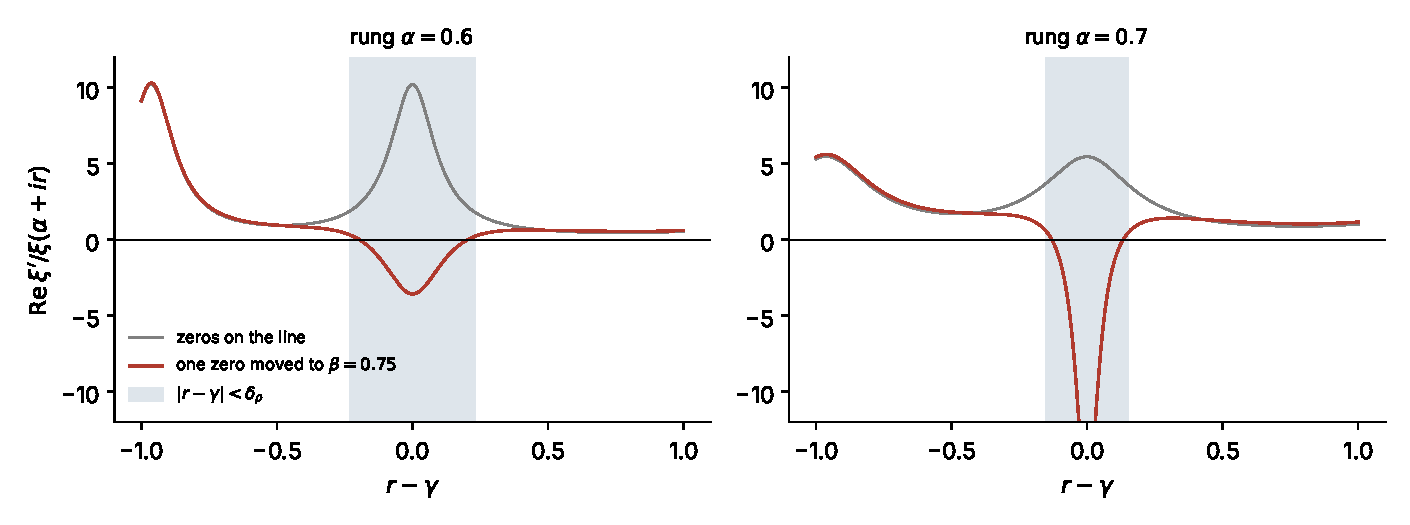
\includegraphics[width=\textwidth]{fig/v3/dz_localization.pdf}
\caption{A hypothetical zero moved off the line. The zero near height $999.79$ is replaced by the pair $\beta=0.75$ and $0.25$. Grey: $v_\alpha(r)$ with all zeros on the line, on the levels $\alpha=0.6$ (left) and $0.7$ (right). Red: after the move. Shaded: the interval $|r-\gamma|<\delta_\rho$ of Theorem~\ref{dz:thm:loc}.}
\label{dz:fig:loc}
\end{figure}
\paragraph{A hypothetical zero (computed).} Moving the zero at $999.79$ to $\beta=0.75$ makes the level $0.6$ negative on $[-0.196,0.203]$ around it, inside the predicted $\delta_\rho=0.229$; the negative Thorin mass is $0.229$, below $m_\rho=0.262$. On the level $0.7$ the negative set is $[-0.130,0.133]$ against $\delta_\rho=0.150$, with mass $0.549$ against $m_\rho=0.590$. The difference is the positive background of the other zeros. Floating point, not certified.

\section{The mass identity}\label{dz:sec:mass}
Integrating \eqref{dz:eq:had} term by term over $0\le r\le R$ gives, for $\alpha>\frac12$ not the real part of a zero,
\[
\mu_\alpha([0,R])=\frac1\pi\int_0^Rv_\alpha\dd r=\frac1\pi\sum_\rho\Big(\arctan\frac{R-\gamma}{\alpha-\beta}+\arctan\frac\gamma{\alpha-\beta}\Big)=\frac1\pi\arg\xi(\alpha+iR),
\]
the argument continued from $\arg\xi(\alpha)=0$ along the level. A zero with $0<\gamma<R$ contributes $+1$ when it is to the left of the level and $-1$ when it is to the right, up to a continuous remainder. A zero to the right comes with its reflection to the left. This is the identity of Proposition~\ref{prop:zerodensity}, which names the remainder.

\begin{theorem}[mass identity]\label{dz:thm:mass}
Let $\alpha=\frac12+\varepsilon>\frac12$ be such that $\xi$ has no zero on the segment from $\alpha$ to $\alpha+iR$, and let $R$ not be an ordinate. Then
\[
\mu_\alpha([0,R])=N(R)-2N(\alpha,R)+E_\alpha(R),\qquad E_\alpha(R)=-\tau_\varepsilon(R),
\]
where $\tau_\varepsilon(R)=\pi^{-1}\Delta\arg\xi$ along the segment from $\alpha+iR$ to $\frac12+iR$. For $\frac12<\alpha\le2$ the remainder is $O(\log R)$ uniformly and is continuous in $\alpha$.
\end{theorem}
\begin{proof}
This is Proposition~\ref{prop:zerodensity} with $\nu(\alpha,R)=N(\alpha,R)$. The change of $\arg\xi$ along a horizontal segment of bounded length at height $R$ is $O(\log R)$ (Titchmarsh~\cite[Section 9.4]{Titchmarsh}), uniformly for $\frac12\le\sigma\le2$; and $\tau_\varepsilon$ is continuous in $\varepsilon$ because $R$ is not an ordinate. The same identity with a rectangle proof is Theorem~\ref{bo:thm:meanvalue}.
\end{proof}
So the total Thorin mass of $[0,R]$ on a level measures $N(\alpha,R)$ to within $O(\log R)$, and each zero to the right removes two units from the count $N(R)$, where localisation only gave less than one.

\begin{corollary}[jump criterion]\label{dz:cor:jump}
Fix $R$ not an ordinate. The function $\alpha\mapsto\mu_\alpha([0,R])$ on $(\frac12,1)$ is continuous except for a jump of $+2$ at each $\alpha=\beta$ for a zero $\beta+i\gamma$ with $0<\gamma<R$ (and $+2m$ for $m$ such zeros). So there are no zeros with $\beta>\frac12$ and $0<\gamma<R$ if and only if the Thorin mass of $[0,R]$ is continuous in the level.
\end{corollary}
The theorem and the corollary both follow from the continuity of $E_\alpha(R)$ and the jump of $2\pi$ in the slope of the logarithmic integral across a zero (Proposition~\ref{prop:littlewood}).

\paragraph{Checks (computed).} Direct integration of $v_\alpha$ agrees with the zero sum to $5\times10^{-6}$: $\mu_{0.6}([0,50])=9.88479$ with $N(50)=10$. On the true zeros $E_\alpha(R)$ lies in $[-0.648,0.886]$ for $100\le R\le2000$ over the levels $\alpha=0.55,0.6,0.75,0.9,1$. With the zero at $999.79$ moved to $\beta=0.75$ and $R=1500.3$, the quantity $\mu_\alpha([0,R])-N(R)$, with $N(R)$ that of the original zeros, is $-0.513$ at $\alpha=0.749$ and $+1.488$ at $\alpha=0.751$: a jump of $2.001$.

\begin{remark}[masking]\label{dz:rem:mask}
The sign of the density on one level does not detect every zero to its right. Take an offending pair with $a=0.05$ on the level $\alpha=0.6$: alone it gives $-16$ at $r=\gamma$. A second pair at the same height with $\beta=0.58$, just to the left of the level, adds $+55.6$, and the density is positive there (computed). So Theorem~\ref{dz:thm:loc} has no converse on one level. The mass identity counts with signs and sees both zeros: moving the level between them shows the jump.
\end{remark}
A positivity argument for RH must therefore control the mass defect $N(R)-\mu_\alpha([0,R])=2N(\alpha,R)+O(\log R)$ and not the negative mass on one level. A proof that this defect is $O(\log R)$ for one $\alpha<1$ and all $R$ would give $N(\alpha,R)=O(\log R)$; a proof that it is $O(R^A)$ is a zero density theorem with exponent $A$.

\section{Littlewood's lemma and the first test}\label{dz:sec:littlewood}
Let $\Phi_R(\sigma)=\int_0^R\log|\xi(\sigma+it)|\dd t$. Then $\Phi_R'(\sigma)=\pi\mu_\sigma([0,R])$ for $\sigma$ not the real part of a zero (Proposition~\ref{prop:littlewood}), and integrating Theorem~\ref{dz:thm:mass} over $\sigma\in[\alpha,\sigma_1]$ gives, for $\frac12<\alpha<\sigma_1$,
\[
2\sum_{\substack{\beta>\alpha\\0<\gamma<R}}\big(\min(\beta,\sigma_1)-\alpha\big)=(\sigma_1-\alpha)N(R)-\frac{\Phi_R(\sigma_1)-\Phi_R(\alpha)}\pi+\int_\alpha^{\sigma_1}E_\sigma(R)\dd\sigma .
\]
This is Littlewood's lemma read on the ladder~\cite[Section 9.9]{Titchmarsh}. It has two consequences, of which only the first direction is a statement about RH. Unconditionally $\Phi_R(\sigma_1)-\Phi_R(\alpha)\le\pi(\sigma_1-\alpha)N(R)+O(\log R)$. Under RH, $\Phi_R(\sigma_1)-\Phi_R(\alpha)=\pi(\sigma_1-\alpha)N(R)+O(\log R)$ for all $\frac12<\alpha<\sigma_1\le1$, and under the quasi Riemann hypothesis with exponent $\theta$ the same holds for $\theta<\alpha$. The converse is false: finitely many zeros to the right of a level, or any set of zeros with total depth $o(\log R)$, satisfy the identity.

Split $\xi=\frac12s(s-1)\pi^{-s/2}\Gamma(\frac s2)\zeta(s)$. By Stirling's formula the Gamma part of $\Phi_R(\sigma_1)-\Phi_R(\alpha)$ equals $\pi(\sigma_1-\alpha)N(R)+O(\log R)$: the Gamma function supplies exactly the mass $N(R)$ per level. Taking $\sigma_1=2$, where $\int_0^R\log|\zeta(2+it)|\dd t=O(1)$, the left side becomes the total depth of the zeros to the right of $\alpha$:
\begin{equation}\label{dz:eq:depth}
\sum_{\substack{\beta>\alpha\\0<\gamma<R}}(\beta-\alpha)=\frac1{2\pi}\int_0^R\log|\zeta(\alpha+it)|\dd t+O(\log R).
\end{equation}
By Jensen's inequality and the mean value $\frac1R\int_0^R|\zeta(\alpha+it)|^2\dd t\to\zeta(2\alpha)$ the depth is at most $\frac R{4\pi}\log\zeta(2\alpha)+o(R)$ for $\frac12<\alpha<1$. Hence $N(\alpha',R)\le\frac{\log\zeta(2\alpha)}{4\pi(\alpha'-\alpha)}R+o(R)$ for $\alpha'>\alpha$, the theorem of Bohr and Landau~\cite{BL14}. Since $N(R)\sim\frac R{2\pi}\log R$, the fraction of Thorin mass lost on any level above $\frac12$ is $O(1/\log R)$. At $R=200.3$ the mean squares of $|\zeta|$ are $2.900$ at $\alpha=0.6$ and $2.179$ at $\alpha=0.75$ (limits $5.592$ and $2.612$), and the resulting bounds on the depth are $17.0$ and $12.4$, against the true value $0$ (computed).

The next classical input is Carlson's method of 1920 (Titchmarsh~\cite[Chapter 9]{Titchmarsh}). Multiply $\zeta$ by the M\"obius mollifier $M_X(s)=\sum_{n\le X}\mu(n)n^{-s}$, the combination that turned Chebyshev's Gamma ratios into $e^w/(1+w)$ (Theorem~\ref{ct:thm:mobius}). Zeros of $\zeta$ are zeros of $\zeta M_X$, so \eqref{dz:eq:depth} holds with $\zeta M_X$ on the right (the zeros of $M_X$ added on the left only help), and $\log|1+g|\le\Re g+\frac12|g|^2$ with $g=\zeta M_X-1$ replaces Jensen. The depth is then controlled by the mean square of $\zeta M_X-1$, which is small:
\begin{center}
\small
\begin{tabular}{@{}cccccc@{}}
\toprule
$X$ & $1$ & $5$ & $20$ & $100$ & $200$\\
\midrule
$\alpha=0.6$ & $1.912$ & $1.088$ & $0.667$ & $0.491$ & $0.397$\\
$\alpha=0.75$ & $1.196$ & $0.457$ & $0.192$ & $0.089$ & $0.058$\\
\bottomrule
\end{tabular}
\end{center}
The table gives the mean of $|\zeta M_X-1|^2$ over $0\le t\le200.3$ (computed). Carlson's argument gives $N(\alpha,R)\ll R^{4\alpha(1-\alpha)+\varepsilon}$; we have not rederived the exponent here. Ingham's exponent needs in addition a bound for $\zeta$ on the critical line, and Guth and Maynard \cite{GM26} need large value estimates for Dirichlet polynomials. So the route reproduces the theorems of 1914 and 1920 with the book's objects, and will not pass the density hypothesis without a new mean value estimate. What the Thorin side adds is positivity structure: by Theorem~\ref{dz:thm:loc} the integrand of $\Phi_R'$ is positive off the defect intervals, a constraint the mean value methods do not use.

\section{How far a level can see}\label{dz:sec:res}
The positive background of the zeros on the line can hide a zero to its right, as a second pair did in Remark~\ref{dz:rem:mask}.
\begin{proposition}[resolution of a level]\label{dz:prop:res}
Let $\rho$ be an offending zero for the level $\alpha$, with $a=\beta-\alpha$, $b=\alpha+\beta-1$, and let $H>0$. Suppose $\rho$ and its reflection are the only zeros with $|\gamma'-\gamma|<H+\frac12$ that are offending or reflections of offending zeros. If
\[
ab>\frac{2(1+H^2)}{L_H(\gamma)-2},
\]
where $L_H(\gamma)$ is the bound of~\eqref{dz:eq:count} for the number of zeros in a window of half width $H$, minimised over centres within $\frac12$ of $\gamma$ (and $L_H(\gamma)>2$), then $v_\alpha(r)>0$ for all $|r-\gamma|<\frac12$: the zero produces no negative Thorin density on the level $\alpha$.
\end{proposition}
\begin{proof}
The pair contributes at least its minimum $P(0)=-(b-a)/(ab)=-2c/(ab)$. The other zeros in the window, at least $L_H-2$ of them, each contribute at least $c/(4c^2+H^2)\ge c/(1+H^2)$ by Lemma~\ref{dz:lem:other}, and everything outside the window is nonnegative.
\end{proof}
Since $L_H(\gamma)\sim\frac H\pi\log\gamma$, the condition reads $ab\gg1/\log\gamma$: at great height a level sees only the zeros within a distance of order $1/((\alpha-\frac12)\log\gamma)$ to its right, and the exceptional set $X_\alpha$ is controlled by the zeros in a thin strip $\alpha<\beta<\alpha+\eta(\gamma)$, not by all of $N(\alpha,R)$. The ladder as a whole still sees every zero, because a zero is visible from the levels just below it, and the mass identity sees every zero from every level.

Two qualifications. First, the proposition is asymptotic in an extreme sense. Because $ab<\frac14$, the best $H$ gives thresholds of $1.71$ at $\log\gamma=30$, $0.313$ at $\log\gamma=100$ and $0.088$ at $\log\gamma=300$ (computed from~\eqref{dz:eq:count}), so it says nothing below about $e^{120}$. Second, the true background is smaller than its average. With the zero near $999.79$ removed, the background at its own ordinate is $0.234$ on the level $0.6$, $0.568$ on $0.75$ and $0.863$ on $0.9$, against a mean value $\frac12\log\frac r{2\pi}=2.5$ (computed): neighbouring zeros repel, so the place where a zero sits is a place where the background is low. In the experiment a zero moved anywhere in $\alpha<\beta<1$ remained visible on all three levels. The heuristic size of the background at a zero is $c\sum_{\gamma'\ne\gamma}(\gamma-\gamma')^{-2}\approx\frac c{12}\log^2\frac\gamma{2\pi}$, which would put the true threshold at $ab\approx24/\log^2\frac\gamma{2\pi}$, reached only for $\gamma>10^5$ (heuristic).

\section{Above the quasi Riemann half plane}\label{dz:sec:qrh}
The half plane $\frac78$ is the theorem of \cite{OAI26a} (Section~\ref{qrh:sec:claims}). We state its consequence for the Thorin density.
\begin{theorem}[by \cite{OAI26a}]\label{dz:thm:qrh}
By the theorem of \cite{OAI26a}, $\zeta(s)\ne0$ for $\Re s>\frac78$. Then $N(\alpha,T)=0$ for every $\alpha>\frac78$ and every $T$, so $v_\alpha(r)>0$ and $v_\alpha(r)\ge b_\alpha$ for every $r\ge0$: both the uncompensated and the compensated Thorin density are nonnegative at every height on every level above $\frac78$.
\end{theorem}
\begin{proof}
There are no offending zeros, so Theorem~\ref{dz:thm:loc} applies at every $r$. For the compensated levels, Proposition~\ref{ct:prop:qrh} with $\theta=\frac78$ gives $v_\alpha\ge b_\alpha$ for $\alpha>\frac78$.
\end{proof}
The levels $\frac12<\alpha\le\frac78$ remain governed by Theorem~\ref{dz:thm:loc}. In the language of this chapter, the theorem of \cite{OAI26a} says that the negative Thorin mass vanishes on the upper eighth of the ladder, and RH says that it vanishes everywhere.

\section{What this does and does not do}\label{dz:sec:limits}
The theorems are unconditional. Theorem~\ref{dz:thm:qrh} rests on \cite{OAI26a}. They are the classical zero density theorems in Thorin language, and Theorem~\ref{dz:thm:loc} contains no new arithmetic: its measure bound is Theorem~\ref{bo:thm:negset}, and the vanishing fraction of negative mass is Theorem~\ref{ag:thm:almost}. What is added here is the dictionary with explicit constants.
\begin{itemize}
\item Each zero to the right of the level $\alpha$ costs less than one unit of Thorin mass, within distance $\frac12$ of its ordinate (Lemma~\ref{dz:lem:pair}).
\item Conversely, negative Thorin mass on the level $\alpha$ near height $\gamma$ certifies a zero to the right of $\alpha$ near $\gamma$.
\item RH says that the negative part vanishes on every level. The density hypothesis implies that its mass up to height $R$ is $O(R^{2(1-\alpha)+\varepsilon})$.
\end{itemize}
To reach RH it is not enough to show that the Gamma side of the budget identity dominates on average, since that is already true and is what Theorem~\ref{dz:thm:comp} uses. One must show that the defects cannot exist. The honest intermediate target is a bound on the total negative Thorin mass that beats the zero density exponents, which would be a new theorem about zeros.

\begin{problem}\label{dz:op:corr}
Replace the crude background bound in Proposition~\ref{dz:prop:res} by one that uses the pair correlation of the zeros, and decide whether the true resolution of a level is of order $1/\log\gamma$ or $1/\log^2\gamma$.
\end{problem}
\begin{problem}\label{dz:op:carlson}
Carry out Carlson's argument in the notation of this chapter and obtain a mass defect of order $R^{4\alpha(1-\alpha)+\varepsilon}$ with explicit constants, as a companion to Theorem~\ref{dz:thm:comp}.
\end{problem}
\begin{problem}\label{dz:op:pos}
On the complement of the defect intervals $v_\sigma(t)>0$, so $\log|\xi(\sigma+it)|$ increases in $\sigma$ there. Does this one sided information improve the mean value of $\log|\zeta M_X|$ beyond what the mean square gives? It is the only place where the Thorin structure could add to the classical method.
\end{problem}
